	\documentclass[letterpaper, 11pt]{article}
\usepackage{comment} % enables the use of multi-line comments (\ifx \fi) 
\usepackage{lipsum} %This package just generates Lorem Ipsum filler text. 
\usepackage{fullpage} % changes the margin

\usepackage{fancyhdr} % Required for custom headers
\usepackage{lastpage} % Required to determine the last page for the footer
\usepackage{extramarks} % Required for headers and footers
\usepackage{mdframed}
\usepackage{caption}
\usepackage{subcaption}
\usepackage{float}
\usepackage{array}
\usepackage{soul}
\usepackage{amsmath}
\usepackage{graphicx} % Required to insert images
\usepackage{multicol}
\usepackage{enumitem}
\usepackage{amssymb,bm}
\usepackage{verbatim,eufrak,hyperref,bbm}
\usepackage{titlesec}
\usepackage{listings}

%%%%% TEMPLATE-SPECIFIC FORMATTING %%%%%
%\usepackage{fourier}
\usepackage[adobe-utopia]{mathdesign}
\titleformat{\section}
  {\normalfont\fontsize{12}{15}\bfseries}{\thesection.}{1em}{}
  \titleformat{\subsection}[runin]{\normalfont}{\thesubsection}{3pt}{}
%\usepackage[T1]{fontenc}

%----------------------------------------------------------------------------------------
%	NAME AND CLASS SECTION
%----------------------------------------------------------------------------------------

\newcommand{\hmwkTitle}{Final \ Review\ Problems} % Assignment title
\newcommand{\hmwkClass}{CME\ 100\ ACE} % Course/class
\newcommand{\hmwkAuthorName}{T Anderson} % Your name
\newcommand{\hmwkAuthorEmail}{timmya@stanford.edu} % Your email

% Set up the header and footer
\pagestyle{fancy}
\lhead{} % Top left header
\chead{} % Top center header
\rhead{} % Top right header
\lfoot{\hmwkClass\ : \hmwkTitle} % Bottom left footer
\cfoot{Page\ \thepage\ of\ \pageref{LastPage}} % Bottom center footer
\rfoot{\hmwkAuthorName} % Bottom right footer
\renewcommand\headrulewidth{0pt} % Size of the header rule
\renewcommand\footrulewidth{0.4pt} % Size of the footer rule


% Math commands
\DeclareMathOperator*{\argmin}{arg\,min}
\DeclareMathOperator*{\argmax}{arg\,max}
\allowdisplaybreaks

% Margins
\topmargin=-0.45in
\evensidemargin=0in
\oddsidemargin=0in
\textwidth=6.5in
\textheight=9.0in
\headsep=0.25in 

\setlength{\parindent}{0pt} % Set indent to zero

\begin{document}

%\thispagestyle{empty}
\noindent
\normalsize 
%\hmwkAuthorName 
\hmwkClass \hfill June\ 10,\ 2017\\
%\hmwkAuthorEmail \\

\begin{center} \Large \textbf{\hmwkTitle} \end{center}

\section{Triple Integrals}
\begin{enumerate}
\item (TC 15.6 \#14) Find the center of mass and moment of inertia about the x-axis of a thin plate bounded by the curves $x = y^2$ and $x = 2y - y^2$ with density $\delta(x,y) = y + 1$.


\item (TC 15.7 \#16) Find the volume of the shape in the following figure. 
\begin{figure}[H]
\centering 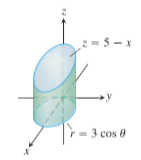
\includegraphics[width=0.15\columnwidth]{finalReviewImgs/TC157_16.png}
\end{figure}



\item (TC 15.7 \#33) Find the volume of the solid between the sphere $\rho = \cos \phi$ and hemisphere $\rho = 2, z \geq 0$. 

\end{enumerate}

\section{Generalized Coordinate Transform}
\begin{enumerate}
\item (TC 15,8 \#2) Find the value of the Jacobian $\partial(x,y)/\partial (u,v)$ for the system:
\begin{gather*}
u = x + 2y \\
v = x - y
\end{gather*}


\item (TC 15.8 \#14) Evaluate the following integral:
\[ \int_0^2 \int_{y/2}^{(y+4)/2} y^3 (2x - y )e^{(2x - y)^2} dx dy \]


\end{enumerate}

\section{Line Integrals}
\begin{enumerate}
\item (TC 16.1 \#12) Evaluate $\int_C \sqrt{x^2 + y^2} ds$ along the curve $\bm{r}(t) = 4\cos t \bm{i} + 4 \sin t \bm{j} + 3t \bm{k}$ for $-2\pi \leq t \leq 2\pi$. 



\item (TC 16.1 \#28) Evaluate $f(x,y) = \frac{x + y^2}{\sqrt{1 + x^2}}$ over the curve $C : y = x^2/2$ from $(1,1/2)$ to $(0,0)$. 


\end{enumerate}

\section{Work}
\begin{enumerate}
\item (TC 16.2 \#20) $\bm{F} = 2y\bm{i} + 3x \bm{j} + (x + y)\bm{k}$ over $\bm{r}(t) = \cos t \bm{i} + \sin t \bm{j} + (t/6)\bm{k}$, $0 \leq t \leq 2 \pi$. 



\item (TC 16.3 \#8) Find the work done by the field $\bm{F} = (y + z)\bm{i} + (x + z) \bm{j} + (x + y) \bm{k}$ when moving on a linear path from $(0,0,0)$ to $(2,4,5)$. 


\item (TC 16.3 \#28) Find the potential function for $\bm{F} = e^x \ln y \bm{i} + \left( \frac{ e^x}{y} + \sin z\right) \bm{j} + y\cos z \bm{k}$. 


\end{enumerate}

\section{Flux}
\begin{enumerate}
\item (TC 16.2 \#32) Find the flux of the field $\bm{F} = x^2 \bm{i} + y^2 \bm{j}$ about the closed semicircular path of radius 2 in the upper half plane. 


%\item (TC 16.2 \#36) Find the flux of $\bm{F} = (x + y) \bm{i} - (x^2 + y^2)\bm{j}$ across the triangle with vertices $(1,0)$, $(0,1)$, and $(-1,0)$.  
%
%\par \textbf{Solution:} Here we need to split the flux calculation up into each of the three edges. We do this because we cannot construct a clean (i.e. differentiable) parameterization that traverses the entire path. Doing this:
%\begin{align*}
%C_1: \bm{r}(t) &= (1-t)\bm{i} + t\bm{j}, \; 0 \leq t \leq 1 \\
%\text{Flux}_1 &= \int 
%\end{align*}


\end{enumerate}

\section{Green's Theorem}
\begin{enumerate}
\item (TC 16.4 \#11) Find the circulation and flux of $\bm{F} = x^3 y^2 \bm{i} + \frac{1}{2} x^4 y \bm{j}$ about the path in the following figure:
\begin{figure}[H]
\centering 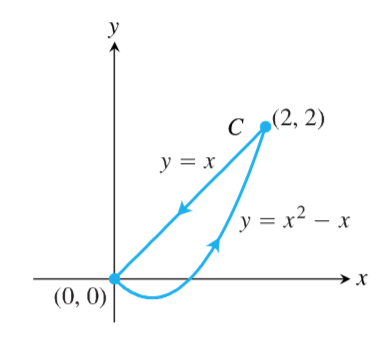
\includegraphics[width=0.2\columnwidth]{finalReviewImgs/TC164_11.png}
\end{figure}

\item (TC 16.4 \#12) Find the circulation and flux of the field $\bm{F} = \frac{x}{1 + y^2} \bm{i} + \tan^{-1}y \bm{j}$. about the unit circle centered at the origin. 



\end{enumerate}

\section{Surface Integrals}
\begin{enumerate}
\item (TC 16.5 \#38) Find the area of the band cut from the paraboloid $x^2 + y^2 - z = 0$ by the plans $z = 2$ and $z = 6$. 


\item (TC 16.6 \#8) Integrate $H(x,y,z) = yz$ over the part of the sphere $x^2 + y^2 + z^2 = 4$ that lies above the cone $z = \sqrt{x^2 + y^2}$. 


%\item (TC 16.6 \#42) Find the area of the cap cut from the sphere $x^2 + y^2 + z^2 = 2$ by the cone $z = \sqrt{x^2 + y^2}$. 


\end{enumerate}

\section{Flux in 3D}
\begin{enumerate}
\item (TC 16.6 \# 22) Find the outward flux of $\bm{F} = x \bm{i} + y \bm{j} + z \bm{k}$ across the sphere of radius 1. 



\end{enumerate}

\section{Stokes' Theorem}
\begin{enumerate}
\item (TC 16.7 \#2) Find the circulation of $\bm{F} = 2y \bm{i} + 3x \bm{j} - z^2 \bm{k}$ about the circle of radius 3 in the $(x,y)$ plane centered at the origin in the counterclockwise direction. 


\item (TC 16.7 \#18) Find the flux of the curl of $\bm{F} = y^2 \bm{i} + z^2 \bm{j} + x \bm{k}$ across the surface $\bm{r}(\phi,\theta) = 2 \sin \phi \cos \theta \bm{i} + 2 \sin \phi\sin \theta\bm{j} + 2\cos \phi \bm{k}$, $ 0 \leq \phi \leq \pi/2$, $0 \leq \theta \leq 2 \pi$. 

\end{enumerate}

\section{Divergence Theorem}
\begin{enumerate}
\item (TC 16.8 \#6) Find the outward flux of $\bm{F} = x^2 \bm{i} + y^2 \bm{j} + z^2 \bm{k}$ across the boundary of the unit cube in the first octant. 



\item (TC 16.8 \#15) Find the flux of $\bm{F} = (5x^3 + 12xy^2)\bm{i} + (y^3+ e^y\sin z)\bm{j} + (5z^3 + e^y \cos z)\bm{k}$ across the boundary of the volume between the spheres $x^2 + y^2 + z^2 =1 $ and $x^2 + y^2 + z^2 = 2$.


\end{enumerate}



\end{document}